%!TEX root = paper.tex

Before continuing, we need to take a tangent and develop a group of sequences which we will call the $\beta$ group, that will be very useful for developing valitation conditions on a collision sequence. The first sequence in this group is defined below.

\begin{definition}
	Given a collision sequence $\alpha$, define a sequence $\beta^{(0)}$ where each element $\beta^{(0)}_i$ is the number of h's between the $i^{th}$ and $(i+1)^{th}$ v in $\alpha$. From Lemma \ref{lem:interval-ticks}, each element in $\beta^{(0)}$ can be one of two different values, which we will refer to as $\beta^{(0)}_{min}, \beta^{(0)}_{max}$.
\end{definition}

Graphically, $\beta^{(0)}_i$ represents the number of tick marks in each interval. An example sequence is shown in Figure \ref{fig:beta-sequence}.

\begin{figure}[H]
  \begin{center}
    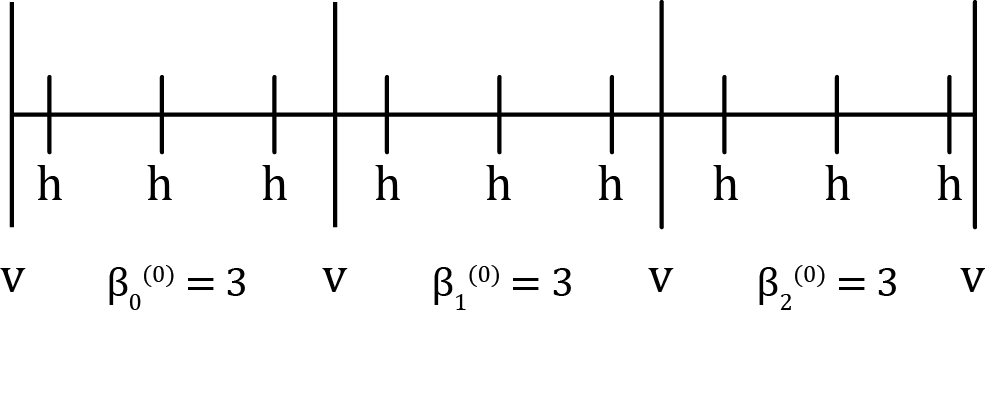
\includegraphics[keepaspectratio, width=4in]{1d_mapping_3}
  \end{center}
  \vspace{-.2in} % corrects bad spacing
  \caption{\label{fig:beta-sequence} An example $\beta^{(0)}$ visual representation.}
\end{figure}

We will the rest of the sequences in the $\beta$ group inductively.

\begin{definition}
  \label{def:beta-definition}
  Given a $j > 0$ and a collision sequence $\alpha$, assume that $\beta^{(j-1)}$ is defined and each element in the sequence is either $\beta^{(j-1)}_{min}$ or $\beta^{(j-1)}_{max}$. The sequence $\beta^{(j)}$ is defined such that each element $\beta^{(j)}_i$ is 1 more than the number of occurrences of $\beta^{(j-1)}_{max}$ between the $i^{th}$ and $(i+1)^{th}$ occurrence of $\beta^{(j-1)}_{min}$ in the $\beta^{(j-1)}$ sequence. From Lemma \ref{lem:interval-ticks}, each element in $\beta^{(j)}$ can be one of two different values, which we will refer to as $\beta^{(j)}_{min}, \beta^{(j)}_{max}$.

	If, for some $j_f$, the length of $\beta^{(j_f-1)}$ is 1, then $\beta^{(j_f-1)}$ is called the terminating $\beta$ sequence, and all subsequent $\beta^{(j)}$ for $j \ge j_f$ are undefined.
\end{definition}

$\beta^{(j)}$ is much simpler to understand visually. A visualization representation is formed using the following rules:

\begin{enumerate}
  \item Divide the number line into regular intervals of length $a_{j}$.
  \item $\beta^{(j-1)}_{min}$ are represented as tick marks on the number line with a regular spacing $a_{j+1}$.
	\item There is exactly one $\beta^{(j-1)}_{min}$ tick mark in each interval.
	\item In each interval, all the $\beta^{(j-1)}_{max}$ terms come before the $\beta^{(j-1)}_{min}$ term.
\end{enumerate}

Then $\beta^{(j)}_i$ is the number of tick marks in each interval. An example $\beta^{(j-1)}$ visual representation is shown in Figure \ref{fig:beta-sequence-j}.

\begin{figure}[H]
  \begin{center}
    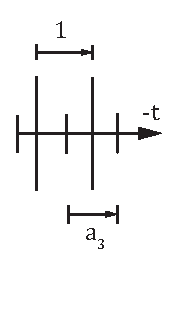
\includegraphics[keepaspectratio, width=4in]{1d_mapping_5}
  \end{center}
  \vspace{-.2in} % corrects bad spacing
  \caption{\label{fig:beta-sequence-j} An example $\beta^{(j)}$ visual representation.}
\end{figure}

Lastly, we will need a new sequence $\delta^{(j)}$ where each element $\delta^{(j)}_i$ is the distance between the $(i \, \beta^{(j)}_{max})^{th}$ tick mark and the beginning of the $i^{th}$ interval in the $\beta^{(j)}$ visual representation. We also include an offset $x_0$ for reasons that will become clear shortly.

\begin{definition}
  $\delta^{(j)}$ is defined more precisely as

  \begin{align}\label{delta_beta}
    \delta^{(j)}_i \coloneqq \begin{cases}
      x_0 \qquad &\text{for} \quad i = 0\\
      i (\beta^{(j)}_{max} * a_{j-1} - a_{j-2}) + x_0 \qquad &\text{for} \quad i \ge 1
    \end{cases}
  \end{align}
\end{definition}

An example $\beta^{(j)}$ sequence is plotted in \ref{fig:a-sequence}, with the $\delta^{(j)}$ values indicated and every $(\beta^{(j)}_{max})^{th}$ tick mark highlighted in red.

\begin{figure}[H]
  \begin{center}
    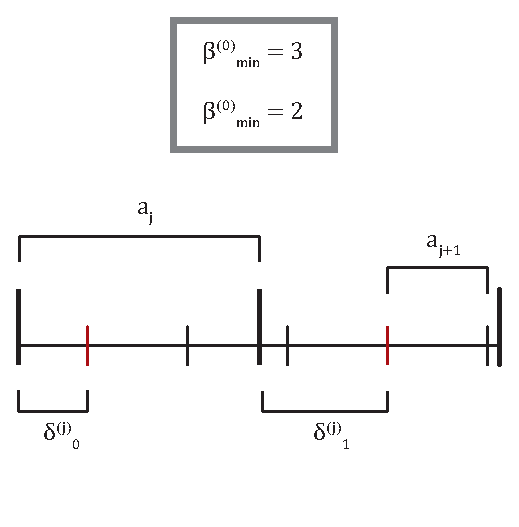
\includegraphics[keepaspectratio, width=4in]{1d_mapping_4}
  \end{center}
  \vspace{-.2in} % corrects bad spacing
  \caption{\label{fig:a-sequence} Example collision sequence with every $(\beta^{(0)}_{max})^{th}$ tick mark highlighted in red.}
\end{figure}

The number of tick marks in the $i^{th}$ interval is thus equal to $\beta^{(j)}_{max}$ plus the number of tick marks included in the $\delta^{(j)}_i$ interval minus the number of tick marks included in the $\delta^{(j)}_{i+1}$ interval. More precisely

\begin{align}\label{eq:beta_i}
  \beta^{(j)}_i = \floor{\delta^{(j)}_i} + \beta^{(j)}_{max} - \floor{\delta^{(j)}_{i+1}}
\end{align}
